\documentclass{article}
\usepackage[utf8]{inputenc}
\usepackage{geometry}
\geometry{letterpaper}
\usepackage[parfill]{parskip}
\usepackage{graphicx}

\usepackage[numbers,sort&compress]{natbib}
\usepackage{amssymb}
\usepackage{amsmath}
\usepackage[english]{babel}   
\usepackage[T1]{fontenc}
\usepackage[autolanguage]{numprint}
\usepackage{color}
\usepackage{subfig}

\usepackage{hyperref}
\usepackage{listings}

\usepackage{tabto}
\usepackage{array}
\usepackage{amsmath}

\usepackage{hyperref}

\usepackage{url}
\usepackage{wrapfig}

\usepackage{amssymb}

\usepackage{caption}

\definecolor{backcolour}{rgb}{0.97,0.95,0.93}

\lstdefinestyle{mystyle}{
    backgroundcolor=\color{backcolour},
}

\author{\Large \textsc{\href{mailto:mohammed.fellaji@supelec.fr}{Mohammed FELLAJI}, \href{mailto:ahmed.benaissa@supelec.fr}{Ahmed BEN AISSA}}}
\date{September, 2020}

\begin{document}

\hypersetup{pdfborder=0 0 0} 		

\makeatletter
  \begin{titlepage}
  \centering
     {\large \textsc{   }}\\
     \vspace{1em}
    \centering
      
\includegraphics[width=0.5 \textwidth]{../figures/LogoCS.png} \\
    \vspace{4cm}
      {\LARGE\textbf{Case Study : Causal Inference}\\  
       \vspace{1em}
       {\large\textbf{
       \textit{\LARGE{Toward Ethical Algorithms ?}}}}\\  
    \vspace{4cm}
    \centering
     {\Large \@author} \\
     \vspace{1em}
        {\Large \textsc{Supervisor : \href{mailto:frederic.pennerath@centralesupelec.fr}{Frédéric PENNERATH}}}\\
        \vspace{3em}
        {\Large \@date} }\\
  \end{titlepage}
 
 
\makeatother

\tableofcontents
%% \listoffigures

%% \newpage
%% \listoftables



%%%%%%%%%%%%%%%%%%%%%%%%%%%%%%%%%%

\newpage
\section{Introduction}
One of the most challenging questions in every problem is the one related to understanding the reason(s) why an action happened and whether or not we can explain it with the information we have at our disposal. Another interesting question one might ask is what would be the outcome if the conditions of the experiment were different ? What would happen if we have more/less information ? What will we get if we change completely the set of inputs ?

When thinking about these questions, having a time machine seems as the perfect solution : we can then repeat the same experiment with different initial conditions and record the outcome in every scenario. A more realistic and possible solution would be to use Causal inference, which aims to estimate the likelihood of an event under static conditions and also under dynamic changing conditions.

While searching about causal inference, one will definitely come across some of the work of Judea Pearl who is credited for developing a theory of counterfactuals and causal inference based on structured models.\footnote{After watching dozens of Judea Pearl lectures and reading many of his papers, we can only recommend doing the same. One of his main ideas is that even if machine learning is shaping millions of industries around the globe, this is done without attention to fundamental theoretical impediments. This might lead machine learning algorithms, very soon, to reach the barriers of impossibility. According to Judea Pearl, the goal is to use the knowledge acquired from causal inference and combine it with the success of machine learning in order to achieve more general models.}

In this document, we will try to study the different literatures about causal inference and collect the results in a simple and yet detailed way. Many papers and book are mentioned in the references section, some were used in writing these document, some are not. Those interested more in the subject may take a look at them.  


\newpage



%%%%%%%%%%%%%%%%%%%%%%%%%%%%%%%%%%

\section{Introductory example : Simpson's Paradox}

Simpson’s paradox, also called Yule-Simpson effect, in statistics, is an effect that occurs when the marginal association between two categorical variables is qualitatively different from the partial association between the same two variables after controlling for one or more other variables.

\begin{figure}[h]
\centering
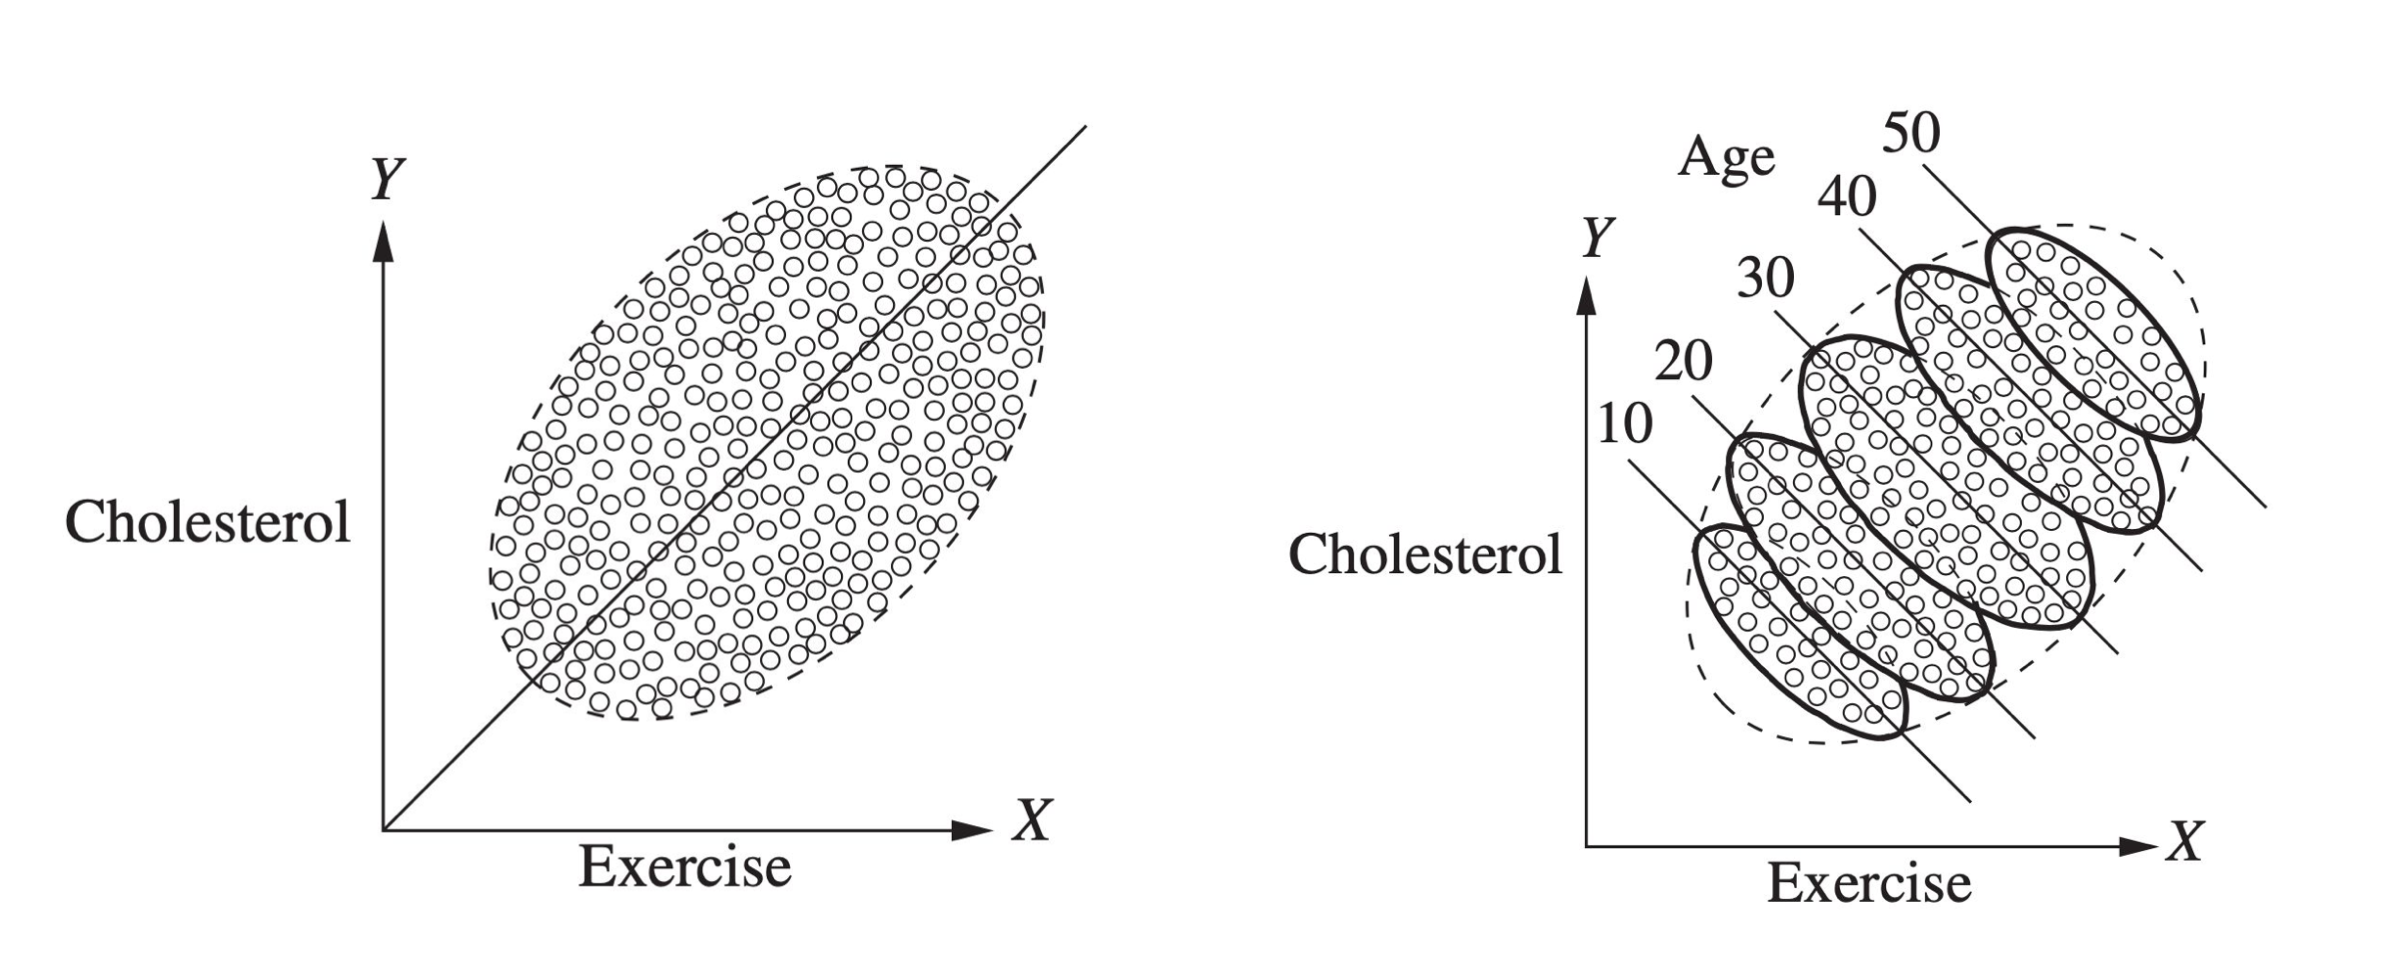
\includegraphics[width=0.7 \textwidth]{../figures/simpson.png}
\caption{Illustration of the Simpson’s Paradox\cite{pearl2016causal}}
\end{figure}

Here is a more detailed illustration of the paradox : 

Imagine we are trying to work out whether a certain drug is an effective treatment for a disease. To decide whether it is effective, we compare people who took the drug (call this x, if someone took the drug, x=1, if not x=0), by examining how many of each recovered from the disease (call this y: y=1 means they got better, y=0 means they did not).

%%%%%%%%%% !!!!
%cite dataset

\begin{figure}[h]
\centering
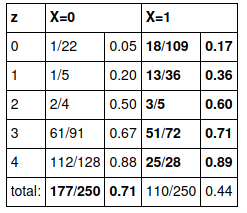
\includegraphics[width=0.4 \textwidth]{../figures/simpson 1.png}
\caption{Results of a study on the effectiveness of a new drug, layered by age group }
\label{fig:studyage}
\end{figure}

When we just look at the last row of Figure~\ref{fig:studyage}, we find that of 250 people who took the drug, 110 recovered ($44 \% $), whereas out of the 250 people who did not take the drug 177 recovered (71\% ). From these results it looks like there is a clear advantage to not taking the drug. Unfortunately, this drug was not administered as part of a random controlled trial. This means that the decision of whether or not to take the drug may have been confounded.

Now let's look at the recovery rate per age group : In every row representing each age group, the patients who were administered the drug got noticeably better.
Thus our conclusion about the drug effectiveness is reversed.

This can be illustrated by Figure~\ref{fig:simpsonexample} above.

\begin{figure}[!tbp]
  \centering
  \subfloat[Positive Correlation]{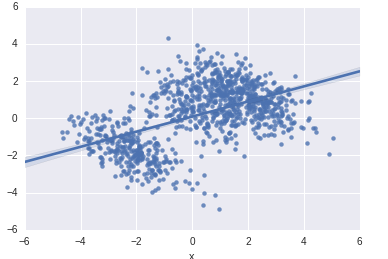
\includegraphics[width=0.44\textwidth]{../figures/simpson2.png}\label{fig:f1}}
  \hfill
  \subfloat[Negative correlation]{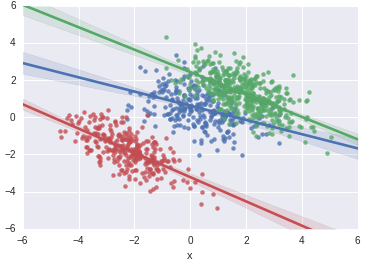
\includegraphics[width=0.44\textwidth]{../figures/simpson 3.png}\label{fig:f2}}
  \caption{Reversal of correlation when a confounding variable, here age, is taken into account}
\label{fig:simpsonexample}
\end{figure}





It is clear now, more often than not, without proper ground knowledge ( here it is medical expertise ), we can ignore confounders such as age, income, .. etc. And without proper randomized experimentation, which is very costly, our understanding of causation can be be contrary to reality.


\newpage

%%%%%%%%%%%%%%%%%%%%%%%%%%%%%%%%%%

\section{Fundamental notions}



%%%%%%%%%%%%%%%%%%%%%%%%%%%%%%%%%%

\subsection{Causation vs Association}

	\subsubsection{Example}

One of the most common phrases in statistics is "correlation does not imply causation". To understand it well, let's take a look a the following example :

\begin{figure}[h]
\centering
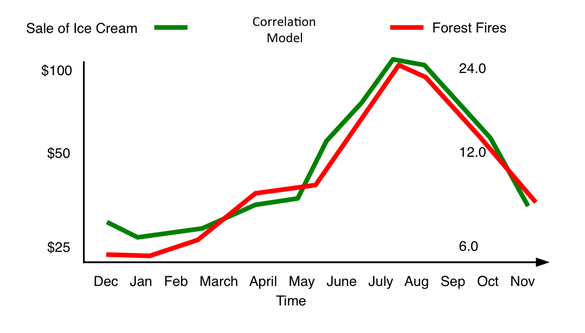
\includegraphics[width=0.6 \textwidth]{../figures/corr_caus.png}
\caption{an example of correlation \href{https://www.decisionskills.com/blog/how-ice-cream-kills-understanding-cause-and-effect}{(source)}}
\end{figure}

Without having any information about what we are trying to model, we might conclude that there is a cause-effect relationship between these two measures. The graph also shows a correlation close to 1 for the two curves. When we start to analyse the data in details, the first thing that comes to our mind is that there is no logical relationship (and thus no cause-effect relationship) between the sale of ice cream and the forest fires. However, we can see clearly in the graph that the values are higher between May and November (with a peak in July) compared to the rest of the year. In fact, the heat is the reason behind forest fires and the sale of ice cream. We can then conclude the following : 

\begin{itemize}
\item[--] a causation between the heat and the sale of ice cream;
\item[--] a causation between the heat and the forest fire;
\item[--] a correlation between the sale of ice cream and the sale of ice cream.
\end{itemize}

This simple example shows us that, in general and without having a good knowledge about the problem, we tend to assume simple correlations between 2 variables when in fact there is a third variable that causes both of them. This is a core idea in causal inference : unlike for correlation, we can not rely only on the distribution of the data, even at the population level, but we also should rely on causal assumption that is always not testable in observational studies.\cite{pearl2010mathematics} 

	\subsubsection{Definitions}
	
The previous example shows a clear difference between causation and correlation. More generally, correlation is a special example of an association concept. The definition of these two concepts is given by Judea Pearl\cite{pearl2010mathematics, pearl2009causal} as follows :

\begin{itemize}
\item[--] An \textbf{associational concept} is any relationship that can be defined in terms of a joint distribution of observed variables. For example: regression, correlation.
\item[--] A \textbf{causal concept} is any relationship that cannot be defined from the distribution alone. One should also rely on causal assumption that explains the different relationships. For example: randomisation, confounding (it will be detailed later).
\end{itemize}


	\subsubsection{The difference between the 2 notions}

To have a better understanding of how causation and association differ, the following example is considered. The goal of a study is to test the effectiveness of a vaccine on a sick population. Let's denote by A the action of injecting the vaccine and by Y the effect of the vaccine on the population. In an association approach, the population will be divided into 2 groups : only one group will be injected with the vaccine. The effectiveness of the treatment is thus measured on the treated population ( $E[Y|A = 1]$ ) and it is also possible to see if the untreated population will be treated without the vaccine ( $E[Y|A = 0]$ ). However, in a causation approach, we suppose that is possible to inject the whole population and study the effect of the vaccine ( $E[Y^{a=1}]$ ) and at the same time, have the same population \textbf{not} injected ( $E[Y^{a=0}]$ ).

\begin{figure}[h]
\centering
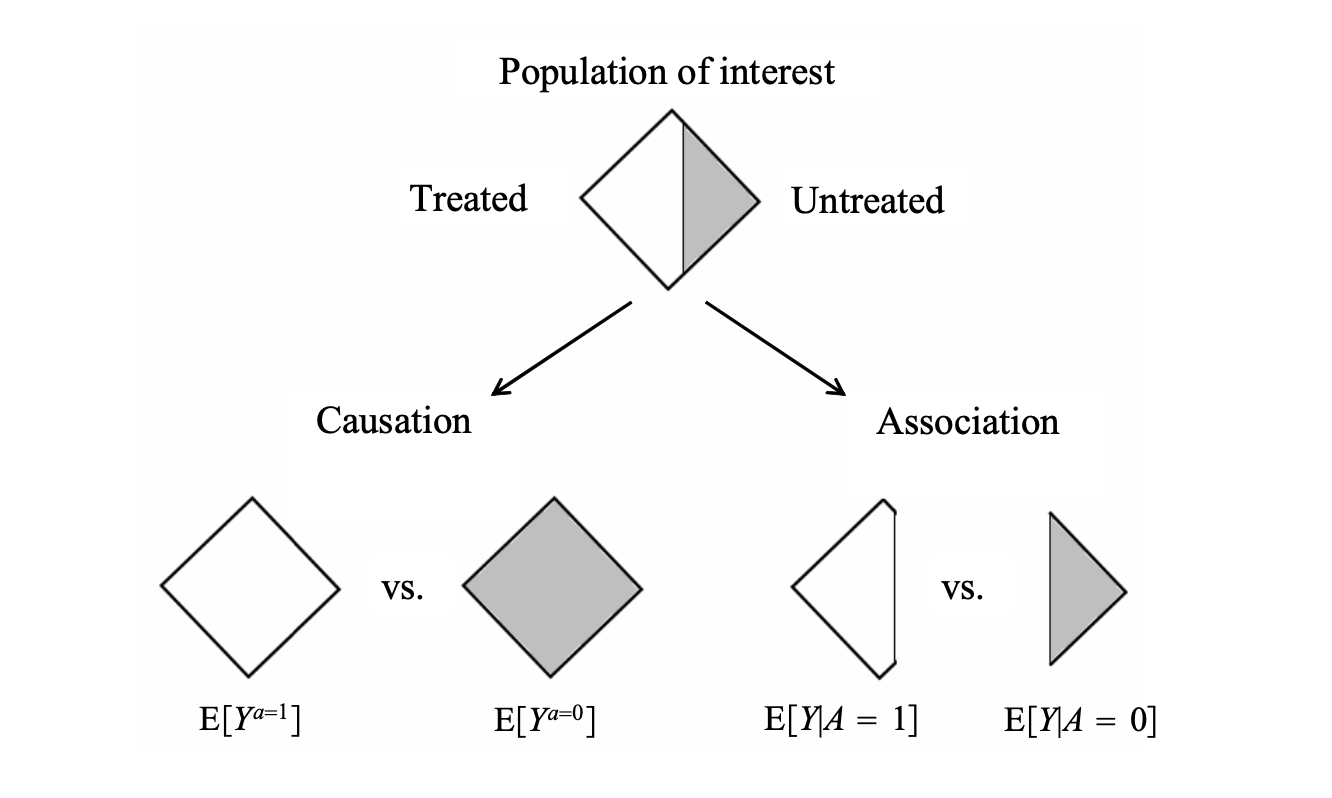
\includegraphics[width=0.6 \textwidth]{../figures/asso_caus.png}
\caption{a visualisation of the difference between causation and association}
\end{figure}

One can see clearly the impossibility of applying in the causation approach : it is impossible to go back in time and inject an individual who was not injected; we can only observe one of the different potential outcomes. Meanwhile, there is some technics so that such an experiment can be possible: randomised experimentation is one example that will be detailed later.

%%%%%%%%%%%%%%%%%%%%%%%%%%%%%%%%%%

\subsection{Counterfactuals}

This is an important concept for causation. Counterfactuals could be defined as the answer to the question "what if ?" or simply as the unobserved outcome. If we consider the previous example in the case of an association, the unobserved outcomes will be the observations of "what if we have injected the proportion of the population that was not injected ?" and of "what if we have not injected the proportion of the population that was injected ?".

%%%%%%%%%%%%%%%%%%%%%%%%%%%%%%%%%%

\subsection{Confounders}

A confounding variable is an unmeasured variable that influences both the supposed cause and the supposed effect. Ignoring the confounder may lead to conclude an association between 2 variables when actually it is not the case. Confounders can also increase the variance or introduce bias.

Different technics exist to reduce the effect of the confounders (random samples, control variable ...)\footnote{An interesting article about confounders could be found at \href{https://www.statisticshowto.com/experimental-design/confounding-variable/}{www.statisticshowto.com}}. However, knowing in advance all the the confounders in the data/model is still very important.

\begin{figure}[h]
\centering
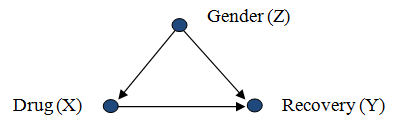
\includegraphics[width=0.5 \textwidth]{../figures/confounding.png}
\caption{An example of a confounding variable : in this example, the Gender is not observed and it is affecting the variables Drug and Recovery}
\end{figure}

 %%%%%%%%%%%%%%%%%%%%%%%%%%%%%%%%%%
 


%\newpage 
%%%%%%%%%%%%%%%%%%%%%%%%%%%%%%%%%%

\section{A mathematical model of causal inference}

In the this section, we suppose the following : 

\begin{itemize}
\item[--] $Y_{i}$ : random variable of the outcome for the "unit" i  (a unit is a physical object, for example, a person, at a particular point in time \cite{rubin2005causal}),
\item[--] N : the number of units,
\item[--] Y : ($Y_{1}$, $Y_{2}$, ..., $Y_{n}$),
\item[--] A : treatment (a treatment is an action that can be applied or withheld from the unit \cite{rubin2005causal}),
\item[--] $Y_{i}^{a}$ : controlled treatment 
\end{itemize}


For simplicity, we assume that the treatment (A) can take only 2 values : \{0,1\}.

%%%%%%%%%%%%%%%%%%%%%%%%%%%%%%%%%%

\subsection{Individual level Causal Effect : ICE}
The ICE is defined as the difference between an individual’s two potential outcomes :
$$ ICE = \delta = Y_{i}^{a=1} - Y_{i}^{a=0} $$


%%%%%%%%%%%%%%%%%%%%%%%%%%%%%%%%%%

\subsection{Average Causal Effect : ACE / Average Treatment Effect : ATE}
The ACE or ATE is the population average of the individual level causal effects :
$$ ACE = E[\delta] = E[Y^{a=1}] - E[Y^{a=0}] $$

ACE is computed over the entire population. If the treatment has a causal effect on the outcome, the value of the ACE will be different than 0 and it will be equal to zero in the other case. This is a mesure of the causation. 
%\newpage
\subsection{Standard estimator : S*}

$$ S^{*} = E[Y^{a=1}|A=1] - E[Y^{a=0}|A=0] $$

S* is computed from the treatment and control groups, and not from the entire population as for the ACE. This is a mesure of the association.

\textbf{\textit{Important special case} : Randomized experimentation}
 
A randomised experiment is when the investigator carried out the action of interest and it wasrandomised because the decision to act on any study subject was made by a random device.Randomisation results in convincing causal inferences, the downsides being mostly finances and logistics.

In the case of randomised experiment, we have the following : 

\begin{itemize}
\item[--] $ E[Y^{a=1}|A=1] =  E[Y^{a=1}|A=0] =  E[Y^{a=1}] $
\item[--] $ E[Y^{a=0}|A=1] =  E[Y^{a=0}|A=0] =  E[Y^{a=0}] $
\end{itemize}

Based on the assertions above, it is easy to prove that a randomised expriment leads to  : $$ ACE = S^{*} $$ which means that it is possible to determine causation from the existing data. This also suppose comparability conditions so that the individuals in both groups are identical.


\newpage
%%%%%%%%%%%%%%%%%%%%%%%%%%%%%%%%%%
 \section{A working example : Evaluating the Econometric Evaluations of Training Programs }
 
 All results are obtained through the python notebook added to the git repository of the project \cite{ourGithub}.
 It is inspired by the models in \cite{lalondeDowhy} , \cite{ijmbarrExample}, and \cite{rugg2Example}.
 
 
 %%%
 
 
 
 
 \subsection{ Dataset}
 
The dataset used to exhibit a model of causal inference is the famous Lalonde datatset, based on the paper : "Evaluating the Econometric Evaluations of Training Programs" by Robert Lalonde\cite{berkeleyExample}.

It studies the effect of education/job training ( the "treatment" ) on the revenue of students after four years in 1978 ( "the outcome" ).

The goal is to estimate the causal effect of the education on revenue, and how it compares to other confounding variables, here it is likely age, education, race and marital status.

\begin{figure}[h]
\centering
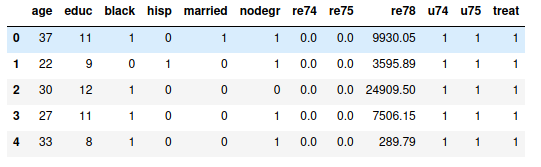
\includegraphics[width=0.8 \textwidth]{../figures/data_overview.png}
\caption{Dataset overview}
\end{figure}


\subsection{ Problem}

\begin{itemize}
    \item Y represents the response, here is is 1978 earnings ("re78")
    \item D represents the treatment: the job training program ("treat")
    \item X represents the confounding variables, here it likely is age, education, race and marital status.
\end{itemize}



\textbf{Problem statement} : How can we disentangle the pure effect of the job training ( Treatment D ) from that of age, education, race, and marital status ( Confounders X ), all have a likely influence on earnings Y ?
 


What we want to know here is the Average Treatment Effect (ATE):
$$ \Delta = ACE = E[Y^{D=1}] - E[Y^{D=0}] $$

However, since we do not have a randomized setting, if we try to estimate this quantity from the row observational distribution, we get:
$$ \Delta^{'} =E[Y \vert  D=1] - E[Y \vert  D=0] \neq \Delta $$

This difference is due to the fact that we do not know, outside a randomized setting, that the treatment D itself is independent from the covariate X. 
However for the rest of this case study, and to be able to use the packages DoWhy and CausalIinference on Python, we make the assumption that D is independent from X.

\subsubsection{Data analysis, Causal discovery}

At first, let look at the statistical description of our database : 

\begin{figure}[h]
\centering
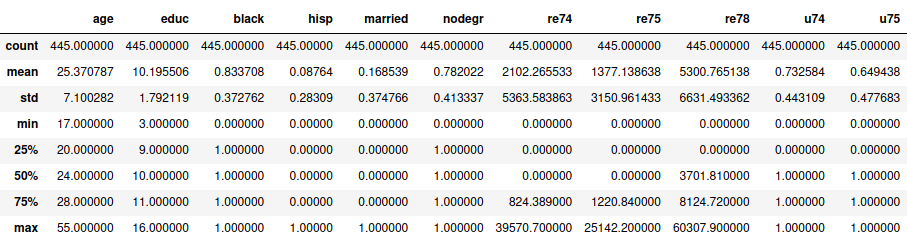
\includegraphics[width=1 \textwidth]{../figures/data_description.png}
\caption{Statistical description of the dataset}
\end{figure}


Let's have a deeper look at how revenue is distributed between the group who got the job training and the one who did not : 

\begin{figure}[h]
\small
\centering
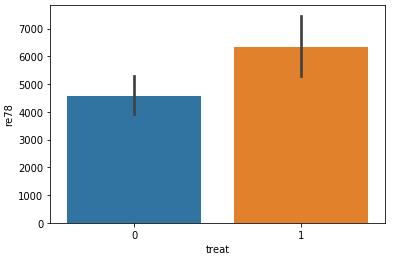
\includegraphics[width=0.5 \textwidth]{../figures/treatment_average_2.png}
\caption{Revenue average for those who followed the job training program versus those who didn't}
\end{figure}


As we could have expected, the group who benefited from the job training program have a higher average revenue after 4 years. However, in order to quantify the net effect of the job training program, we have to check the balance of our data set, and cross-examine the influence of each and every confounder of X.

We start with age (left figure) and education (right figure) represented in Figure~\ref{ref:imbalance} :

\begin{figure}[!tbp]
  \centering
  \subfloat[Age imbalance]{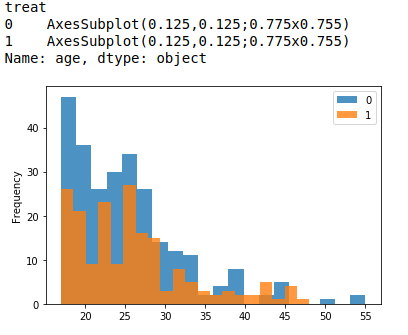
\includegraphics[width=0.44\textwidth]{../figures/age_imbalance.png}\label{fig:f1}}
  \hfill
  \subfloat[education imbalance]{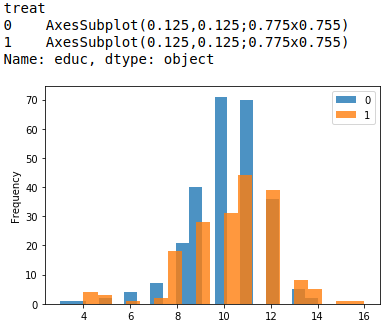
\includegraphics[width=0.44\textwidth]{../figures/education_imbalance.png}\label{fig:f2}}
  \caption{Dataset imbalances}
  \label{ref:imbalance}
\end{figure}



At first look, it is clear that our dataset is imbalanced. This imbalance in age distribution, as well as other confounders, makes drawing any conclusion erroneous. 



\subsubsection{Naive estimate}

At first, let's have a naive estimate of the impact of the job training program on revenue.
We ignore any potential confounder of X. We obtain through the mean formula :
$$ \Delta^{'} = ACE_{0} = E[Y1] - E[Y0]= \$ 1794.34 $$


\subsubsection{Linear Model}

An intuitive approach to the estimating the impact of the confounders X would be the linear model, assuming the law of the revenue Y follows :
$$ Y = \alpha + \beta D + \gamma X
$$
A simple multi-variable linear regression allows us to obtain specific estimate for each and every coefficient.
Using the CausalModel library on python, we compute the mean using the obtained coefficients, and we obtain a rough estimate of the Average Causal Effect : 

%%
\begin{figure}[h]
\small
\centering
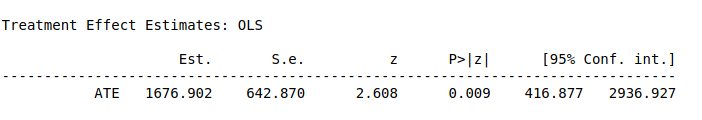
\includegraphics[width=0.8 \textwidth]{../figures/ate_linear_model.png}
\caption{Average job training effect according to the matching model}
\end{figure}



Thus, according to the linear model, the net increase in revenue due to the job training is \$ 1676.90, a significant decrease from the \$1794.34 in the naive model. This decrease is due to X, the confounder variable, being taken into account.

\textbf{However}, the linear model has it limits. First of all, it is heavily influenced with data imbalances. Moreover, the OLS estimator is a simplistic point of view and may not capture all the intricacies of the interaction of the outcome Y with the confounders.

In the next section, we offer a more sophisticated approach, that improves on the linear model.

%\newpage
\subsubsection{A more sophisticated approach : propensity score, stratification and matching}

The \textbf{Propensity Score} is the probability of receiving the treatment, conditional on the covariates.
$$ p(X) = P( D=1 \vert X )$$
It has two main uses : 
\begin{itemize}
    \item Instead of using X as the covariate, $p(X)$ summarises the information contained in X that is relevant to causal inference.
    \item It allows us to drop samples with extreme propensity scores, and to focus on matching on similar samples
\end{itemize}
Both the CausalInference and DoWhy allows for a quick estimation of p(X) using statistical likelihood tests, and for trimming the dataset using this estimation.

\textbf{Stratification} is clustering the samples into layers of similar propensity scores, which allow for more consistent estimations.

\textbf{Matching} estimation exploits the specific distribution within the stratified layers, using nearest-neighbour methods, to improve on the quality of estimates and detect the slightest of effect confounding variables have.

Applying these three methods to our dataset, we obtain the following output to our algorithm: 

\begin{figure}[h]
\small
\centering
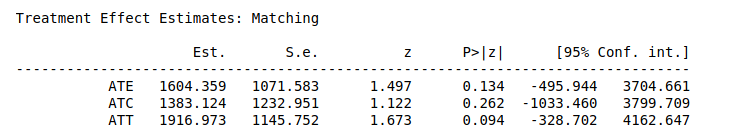
\includegraphics[width=0.8 \textwidth]{../figures/matching_estimate.png}
\caption{Average job training effect according to the matching model}
\end{figure}




The average treatment effect of the job training program is an \$1604 increase in revenue over the following four years. 

\subsubsection{Conclusion}

While our model is a very simplified approach to the causal inference problem, it offers a solid base to build on, using more sophisticated model. 
Deep learning models in particular, as cited in \cite{yao2020survey}, do not assume linearity, which is far more reflective of reality, and allow for better estimation of the Average Causal Effect of a perceived cause on a specific outcome







%%%%%%%%%%%%%%%%%%%%%%%%%%%%%%%%%%

\newpage
\addcontentsline{toc}{section}{References}
\bibliographystyle{ieeetr} % plain : no order -- ieeetr : sorted
\nocite{*}    % print all references
\bibliography{../reference/ref}

\end{document}
